\section{Strategy 4: the direct nine-point obstruction}
\label{sec:ab-core}

Assume all six vertex roles are Vd0, they cover $\partial H$, and exactly
one actual boundary row is supercritical.  Rotate the supercritical index to
$4$.  The strict handoffs from Proposition~\ref{prop:strict-handoffs} obey
\begin{equation}
 x_3<x_2<x_1<x_0<x_5<x_4.
 \label{eq:overview-extreme-chain}
\end{equation}
Put
\[
 a=1-x_3,\qquad b=x_4,\qquad p=1-b,\qquad q=1-a.
\]
Then $a+b>1$, $a^2+ab+b^2<1$, and every selected row has incoming and
outgoing demands at least $p$ and $q$.  This single descent chain is why the
strategy is specific to $N_+=1$.

\subsection{Forcing nine points into the center role}

Let $c_*=c_{\max}(p,q)$ be the exact maximal radial reach for the common
boundary demands.  The six points
\[
 D_i=(1-c_*)V_i\qquad(0\le i\le5)
\]
are excluded from their matching Vd0 role by maximality and openness, from
the adjacent roles by Vd0 locality, and from the remaining roles by the
diameter-one condition.  Thus all six lie in $U_C$, and their convex hull
forces a centered disk $\mathcal D_\eta\subset U_C$.

Three parameter-dependent points $Q_-,Q_0,Q_+$ are then placed on the two
actual neighboring handoff lines.  The unique supercritical row is excluded
by its exact strict frontier; rows $0,1,2$ are excluded by direct vertex
distances; and rows $3,5$ are excluded by the actual handoffs.  Hence these
three points also lie in $U_C$.

\begin{figure}[H]
\centering
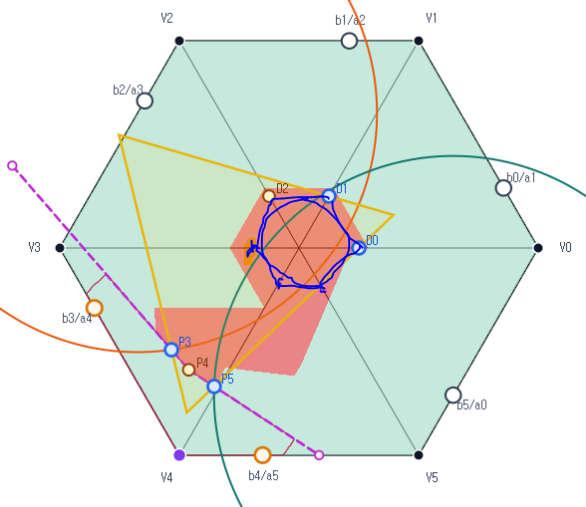
\includegraphics[width=.72\linewidth,keepaspectratio]
  {figures/strategy4_core_case_example.png}
\caption{Author-supplied illustrative Strategy~4 core-case configuration,
not to scale.  The displayed placement is an example only; no exclusion,
forcing, or enclosure inequality is inferred from the picture.}
\label{fig:strategy4-core-case}
\end{figure}

\subsection{Why the witness cannot fit}

For a compact set $K$, let $\Lambda(K)$ be the least side length of a closed
equilateral triangle containing $K$.  The witness-enclosure theorem proves
\[
 \Lambda\!\left(\conv(\mathcal D_\eta\cup
 \{Q_-,Q_0,Q_+\})\right)\ge1.
\]
Its geometric core is a four-cap chain in the support-direction circle.
Adjacent overlaps are analytic; the two mixed overlaps are reduced to exact
integer-polynomial signs and verified by global Bernstein identities.

The nine-point set is compact.  If it lay inside the open unit triangle
$U_C$, positive clearance from the three sides would place it in a closed
equilateral triangle of side strictly below one, contradicting the displayed
lower bound.

\begin{proposition}[Strategy 4 interface]
\label{prop:nine-point-interface}
Strategy~4 closes exactly the zero-gap, all-Vd0, $N_+=1$ rows of
Table~\ref{tab:routing}, for every center class.
\end{proposition}

\begin{proof}
The technical center-independent obstruction is
Theorem~\ref{thm:zero-gap-obstruction}.  In CE0, a missed boundary point
would create a positive center trace, so zero gaps are automatic.  In CE1
or CE2, zero gaps say directly that the six vertex roles cover
$\partial H$.  Appendix Proposition~\ref{prop:ab-core-branches} makes these
two applications explicit.
\end{proof}
